\PassOptionsToPackage{unicode=true}{hyperref} % options for packages loaded elsewhere
\PassOptionsToPackage{hyphens}{url}
%
\documentclass[ignorenonframetext,]{beamer}
\usepackage{pgfpages}
\setbeamertemplate{caption}[numbered]
\setbeamertemplate{caption label separator}{: }
\setbeamercolor{caption name}{fg=normal text.fg}
\beamertemplatenavigationsymbolsempty
% Prevent slide breaks in the middle of a paragraph:
\widowpenalties 1 10000
\raggedbottom
\setbeamertemplate{part page}{
\centering
\begin{beamercolorbox}[sep=16pt,center]{part title}
  \usebeamerfont{part title}\insertpart\par
\end{beamercolorbox}
}
\setbeamertemplate{section page}{
\centering
\begin{beamercolorbox}[sep=12pt,center]{part title}
  \usebeamerfont{section title}\insertsection\par
\end{beamercolorbox}
}
\setbeamertemplate{subsection page}{
\centering
\begin{beamercolorbox}[sep=8pt,center]{part title}
  \usebeamerfont{subsection title}\insertsubsection\par
\end{beamercolorbox}
}
\AtBeginPart{
  \frame{\partpage}
}
\AtBeginSection{
  \ifbibliography
  \else
    \frame{\sectionpage}
  \fi
}
\AtBeginSubsection{
  \frame{\subsectionpage}
}
\usepackage{lmodern}
\usepackage{amssymb,amsmath}
\usepackage{ifxetex,ifluatex}
\usepackage{fixltx2e} % provides \textsubscript
\ifnum 0\ifxetex 1\fi\ifluatex 1\fi=0 % if pdftex
  \usepackage[T1]{fontenc}
  \usepackage[utf8]{inputenc}
  \usepackage{textcomp} % provides euro and other symbols
\else % if luatex or xelatex
  \usepackage{unicode-math}
  \defaultfontfeatures{Ligatures=TeX,Scale=MatchLowercase}
\fi
\usetheme[]{Madrid}
\usefonttheme{professionalfonts}
% use upquote if available, for straight quotes in verbatim environments
\IfFileExists{upquote.sty}{\usepackage{upquote}}{}
% use microtype if available
\IfFileExists{microtype.sty}{%
\usepackage[]{microtype}
\UseMicrotypeSet[protrusion]{basicmath} % disable protrusion for tt fonts
}{}
\IfFileExists{parskip.sty}{%
\usepackage{parskip}
}{% else
\setlength{\parindent}{0pt}
\setlength{\parskip}{6pt plus 2pt minus 1pt}
}
\usepackage{hyperref}
\hypersetup{
            pdftitle={Elucidating gene networks precipitating relapse in CAR T-Cell treated diffuse large B-cell lymphoma},
            pdfauthor={Will Patterson; Bo Hu (Advisor)},
            pdfborder={0 0 0},
            breaklinks=true}
\urlstyle{same}  % don't use monospace font for urls
\newif\ifbibliography
\usepackage{longtable,booktabs}
\usepackage{caption}
% These lines are needed to make table captions work with longtable:
\makeatletter
\def\fnum@table{\tablename~\thetable}
\makeatother
\setlength{\emergencystretch}{3em}  % prevent overfull lines
\providecommand{\tightlist}{%
  \setlength{\itemsep}{0pt}\setlength{\parskip}{0pt}}
\setcounter{secnumdepth}{0}

% set default figure placement to htbp
\makeatletter
\def\fps@figure{htbp}
\makeatother

\usepackage{mathtools}
\usepackage{amssymb}
\usepackage{amsmath}
\usepackage{graphicx}
\AtBeginDocument{\title[DLBCL Multiomics]{Elucidating gene networks precipitating relapse in CAR T-Cell treated diffuse large B-cell lymphoma}}
\titlegraphic{
\includegraphics[width=0.3\paperwidth]{\string images/cclogo.jpg}}

\title{Elucidating gene networks precipitating relapse in CAR T-Cell treated
diffuse large B-cell lymphoma}
\providecommand{\subtitle}[1]{}
\subtitle{A case for multiple CCA and heirarchical tree trimming}
\author{Will Patterson \and Bo Hu (Advisor)}
\date{8/28/2020}

\begin{document}
\frame{\titlepage}

\begin{frame}{Outline}
\protect\hypertarget{outline}{}

\textbf{Hypothesis}: Integration of multi-omics signals will elucidate
gene networks involved in DLBCL relapse after CAR T-cell therapy.

\begin{enumerate}
\item
  \textbf{What}: Diffuse Large B-Cell Lymphoma
\item
  \textbf{Why}: Approximately half of patients with DLBCL treated with
  CAR T-cells will relapse
\item
  \textbf{How}: Multi-omics integration using sparse multiple cannonical
  correlation analysis
\end{enumerate}

\end{frame}

\begin{frame}{What: Diffuse Large B-Cell Lymphoma}
\protect\hypertarget{what-diffuse-large-b-cell-lymphoma}{}

\begin{figure}

{\centering 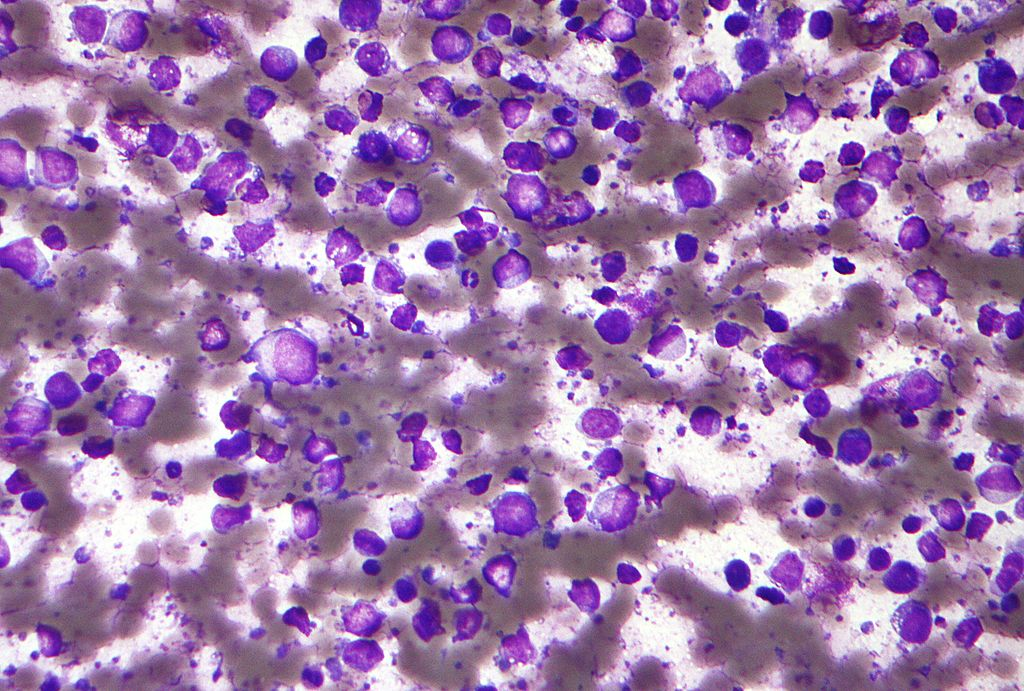
\includegraphics[width=0.45\linewidth]{images/dlbcl_stain} 

}

\caption{Micrograph of DLBCL (Field stain)}\label{fig:unnamed-chunk-1}
\end{figure}

\begin{itemize}
\item
  Most common non-Hodgkin lymphoma (5.6 per 100,000 persons per year),
  arises from mature B lymphocytes
\item
  Average 5-year relative survival rate of 63\% (72\% for all NHL)
\item
  \textbf{Treatment:} R-CHOP/EPOCH \(\rightarrow\) salvage/HCT
  \(\rightarrow\) CAR T-cell
\end{itemize}

\end{frame}

\begin{frame}{Multiple Canonical Correlation Analysis: Definition}
\protect\hypertarget{multiple-canonical-correlation-analysis-definition}{}

\textbf{Canonical Correlation Analysis (CCA)} finds the relationship
between sets of variables by finding their maximally correlated linear
combinations.

\textbf{Given}: \(K\) sets of observations on same \(n\) observations,
\(\textbf{X}_1,...,\textbf{X}_K\) of dimensions \(n \times p_k\), all
standardized to mean zero and SD of one

\textbf{Find}: Weights \(\textbf{w}_1,...,\textbf{w}_k\), where
\(\textbf{w}_k \in \mathbb{R}^{p_k}\), such that the objective function
below is maximized

\begin{block}{Multiple CCA objective function}

\begin{equation} \label{eq:penalized_smcca}
    \text{maximize}_{\textbf{w}_1,...,\textbf{w}_K} \sum_{i<j} \textbf{w}_i^T\textbf{X}_i^T\textbf{X}_j\textbf{w}_j \text{ subject to }||\textbf{w}_i||^2 \leq 1, P_i(\textbf{w}_i) \leq c_i, \forall i \notag
\end{equation}

\begin{center}
(where $P_i$ is the $L_1$ penalty for $i^{th}$ set)
\end{center}

\end{block}

\end{frame}

\begin{frame}{Extension of sparse mCCA to binary outcomes}
\protect\hypertarget{extension-of-sparse-mcca-to-binary-outcomes}{}

Witten and Tibshirani (2009) suggest an extension of sparse mCCA that
allows for the incorporation of a two-class outcome. Their method simply
treats this \(\mathbb{R}^{n\times1}\) matrix as a third data set. Their
objective function takes the form:

\begin{block}{Sparse mCCA objective function with binary variables}

\begin{equation} \label{eq:penalized_smcca_with_binary}
\text{maximize}_{\textbf{w}_1, \textbf{w}_2, \textbf{w}_3} \textbf{w}_1^T\textbf{X}_1^T\textbf{X}_2\textbf{w}_2 +
    \textbf{w}_1^T\textbf{X}_1^T\textbf{y}\textbf{w}_3 +
    \textbf{w}_2^T\textbf{X}_2^T\textbf{y}\textbf{w}_3 \notag \end{equation}
\begin{equation} \text{subject to }||\textbf{w}_i||^2 \leq 1, P_i(\textbf{w}_i) \leq c_i, \forall i \notag
\end{equation}

\end{block}

\end{frame}

\begin{frame}{Extracting gene networks from multiple CCA}
\protect\hypertarget{extracting-gene-networks-from-multiple-cca}{}

Three step process for gene network extraction:

\begin{enumerate}
\item
  Compute the similarity matrix based on the outer products of absolute
  canonical correlation weights.
\item
  Apply hierarchical tree cutting to the similarity matrix and extract
  modules that contain all -omics data types.
\item
  Visualize networks.
\end{enumerate}

\end{frame}

\begin{frame}{Diagnostic Samples Only: Gene Expression}
\protect\hypertarget{diagnostic-samples-only-gene-expression}{}

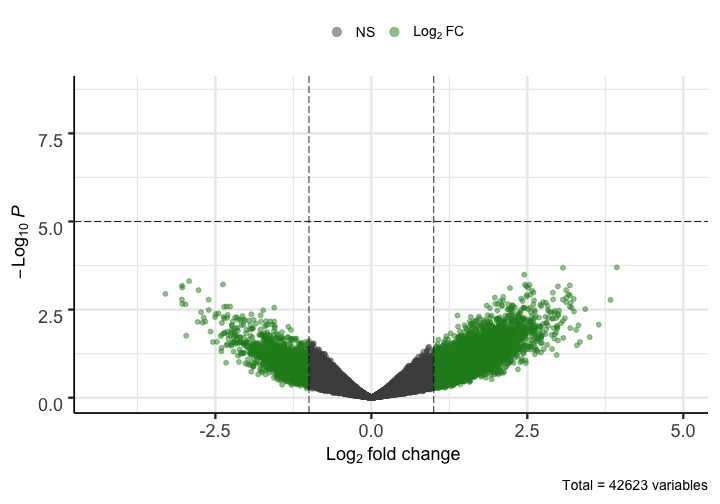
\includegraphics[height=0.85\textheight]{final_presentation_slides_files/figure-beamer/DRR_gene_volcano-1}

\end{frame}

\begin{frame}{Diagnostic Samples Only: Methylation Sites}
\protect\hypertarget{diagnostic-samples-only-methylation-sites}{}

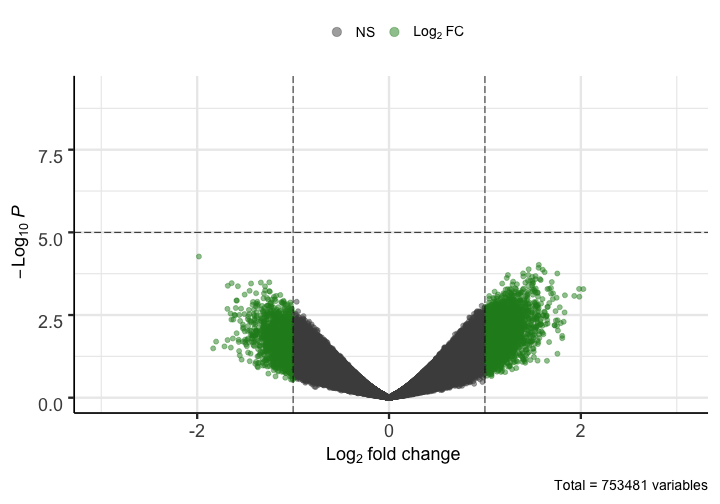
\includegraphics[height=0.85\textheight]{final_presentation_slides_files/figure-beamer/DRR_methyl_volcano-1}

\end{frame}

\begin{frame}{Diagnostic Samples Only: Gene Network Analysis}
\protect\hypertarget{diagnostic-samples-only-gene-network-analysis}{}

\begin{center}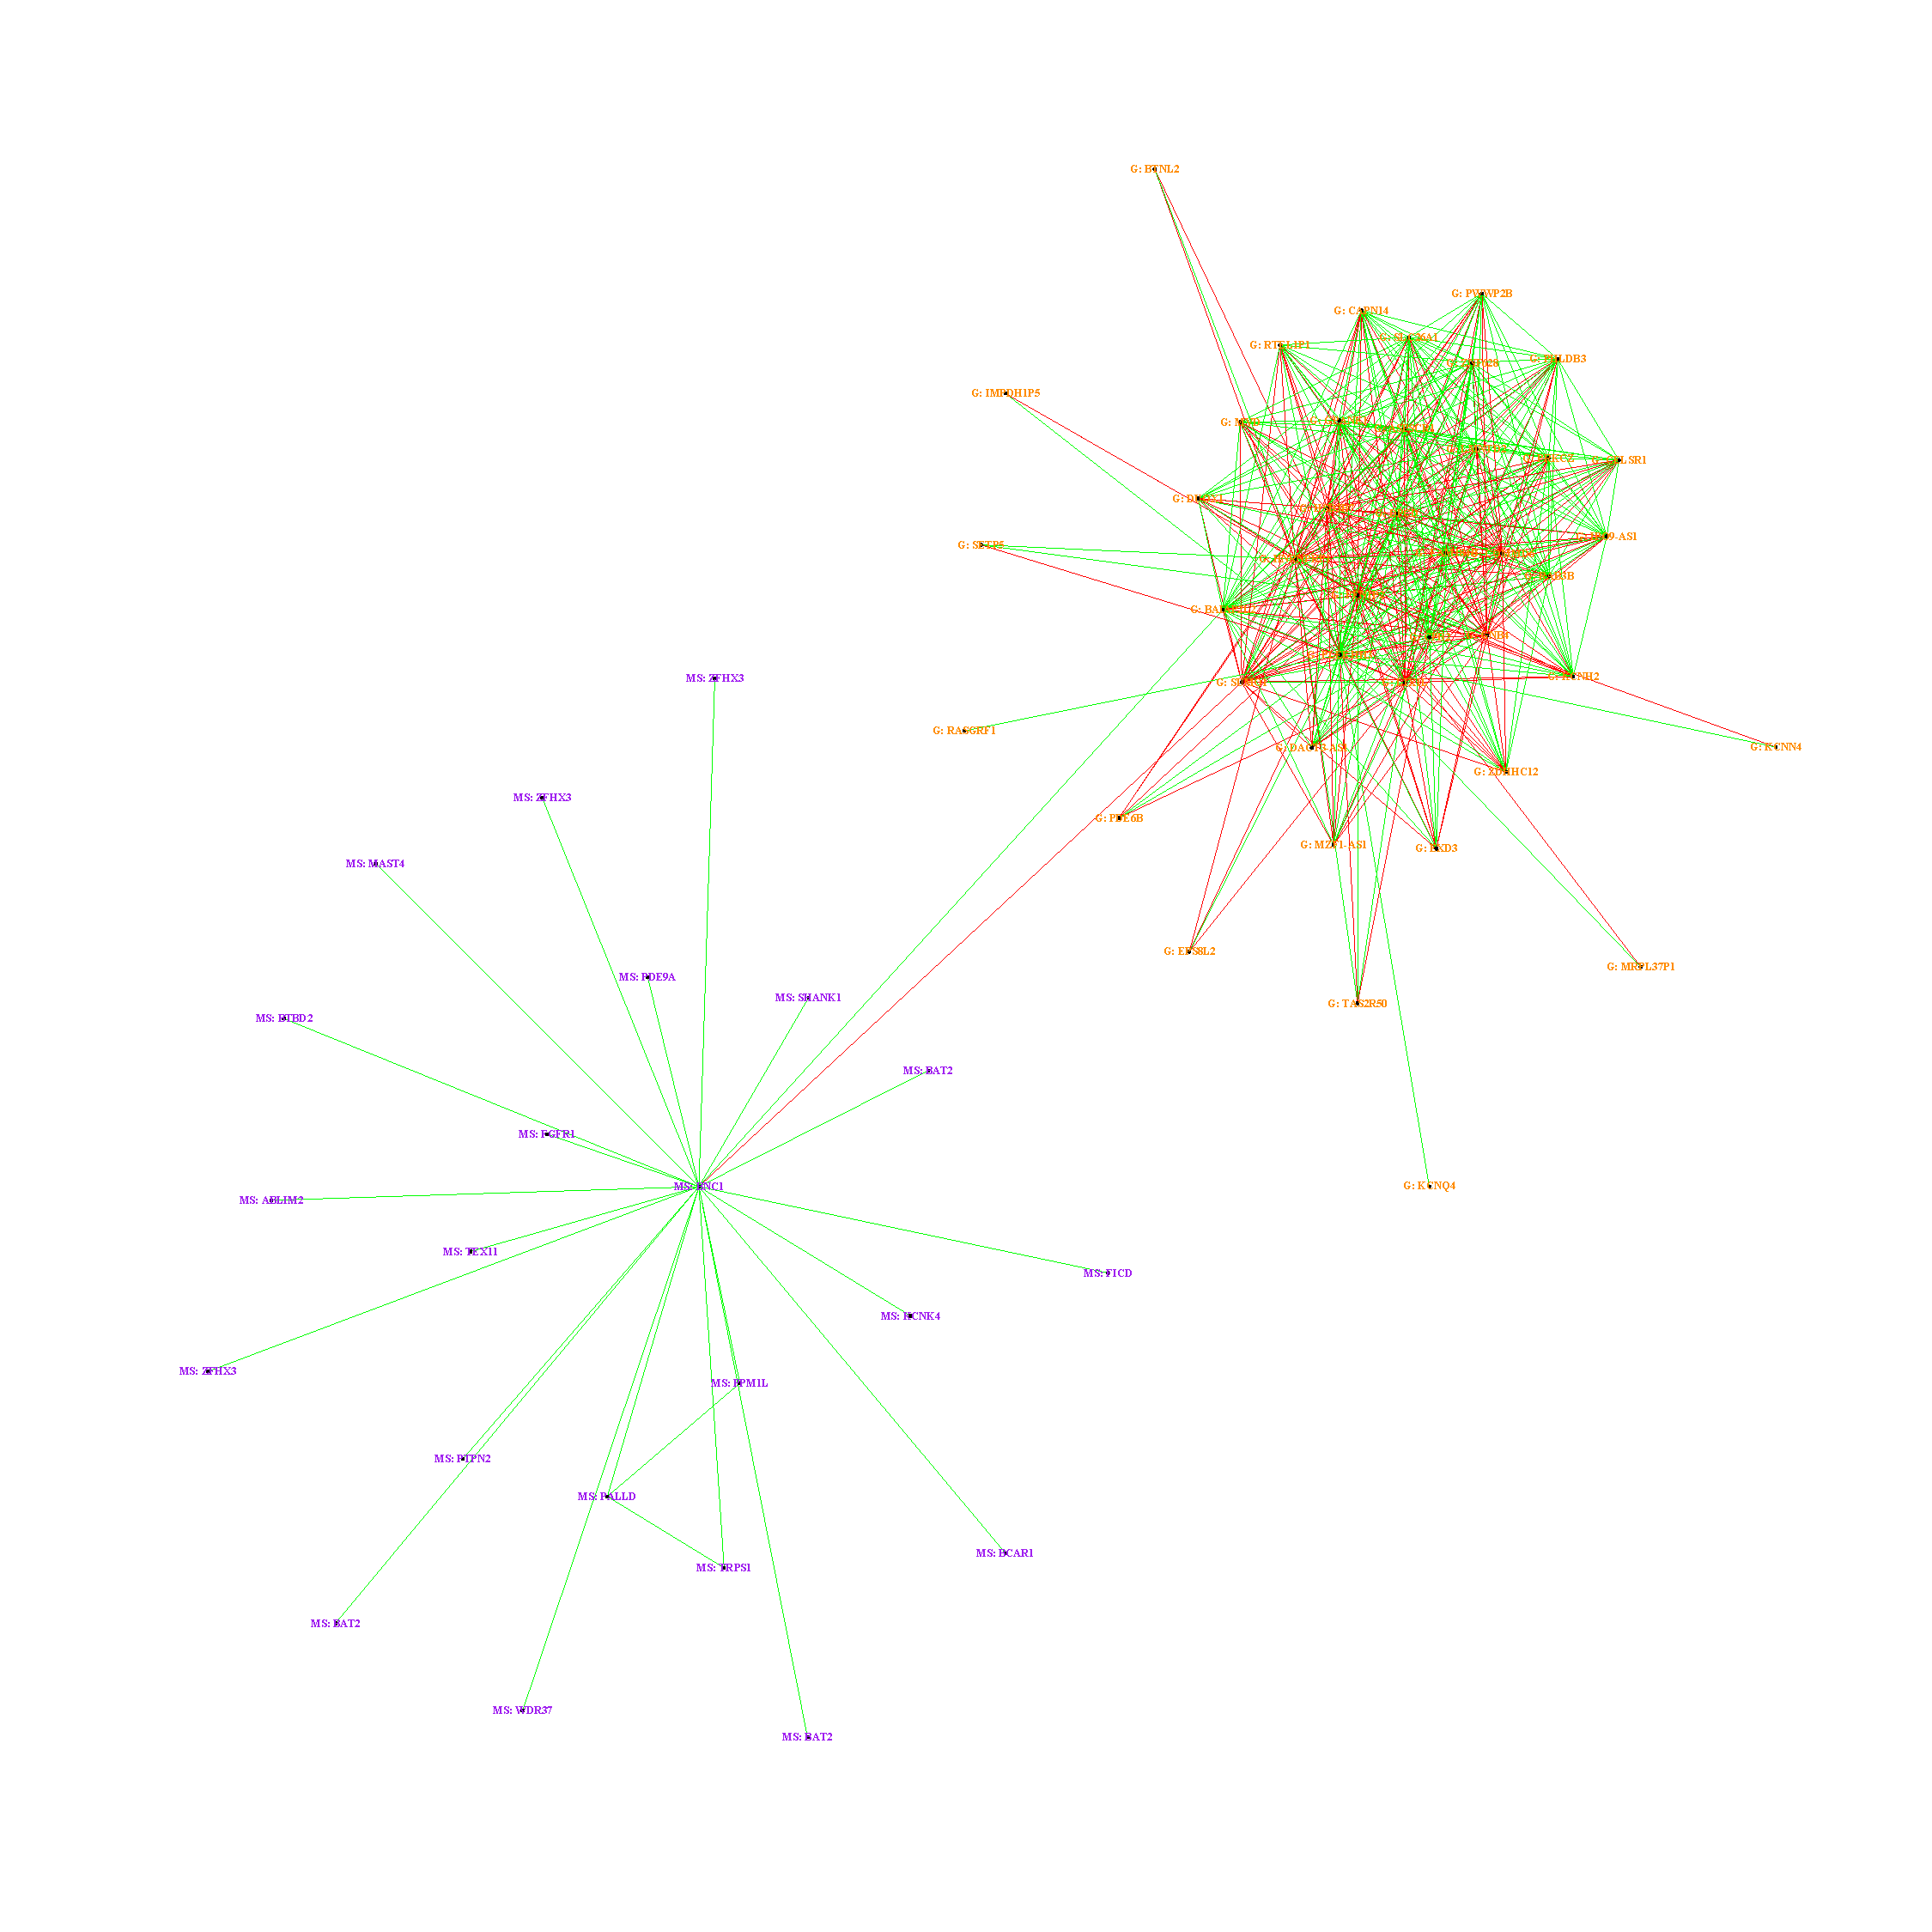
\includegraphics[width=0.7\linewidth]{images/DRRNet1} \end{center}

\end{frame}

\begin{frame}{Diagnostic vs.~Relapsed Patients: Gene Expression}
\protect\hypertarget{diagnostic-vs.relapsed-patients-gene-expression}{}

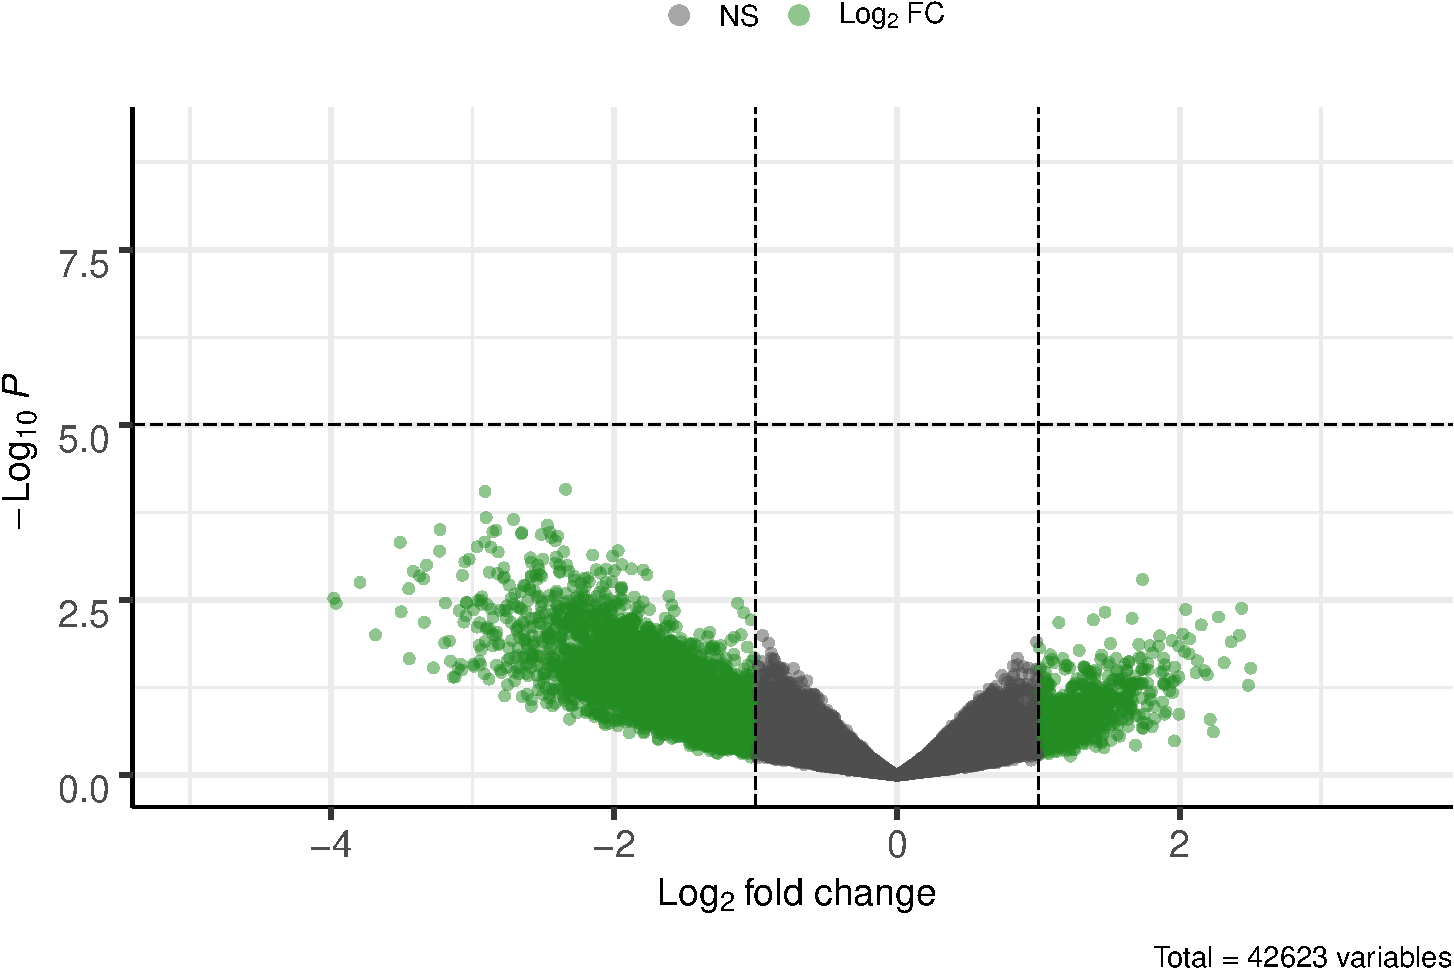
\includegraphics[height=0.85\textheight]{final_presentation_slides_files/figure-beamer/DRDC_gene_volcano-1}

\end{frame}

\begin{frame}{Diagnostic vs.~Relapsed Patients: Methylation Sites}
\protect\hypertarget{diagnostic-vs.relapsed-patients-methylation-sites}{}

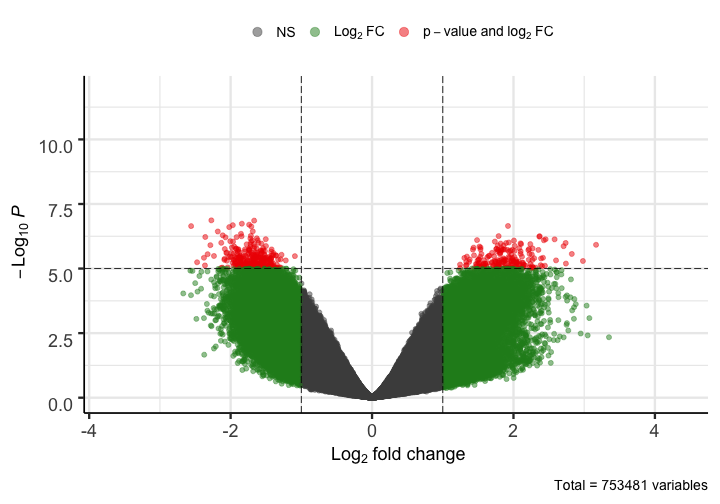
\includegraphics[height=0.85\textheight]{final_presentation_slides_files/figure-beamer/DRDC_methyl_volcano-1}

\end{frame}

\begin{frame}{Diagnostic vs.~Relapsed Patients: Gene Network Analysis}
\protect\hypertarget{diagnostic-vs.relapsed-patients-gene-network-analysis}{}

\begin{center}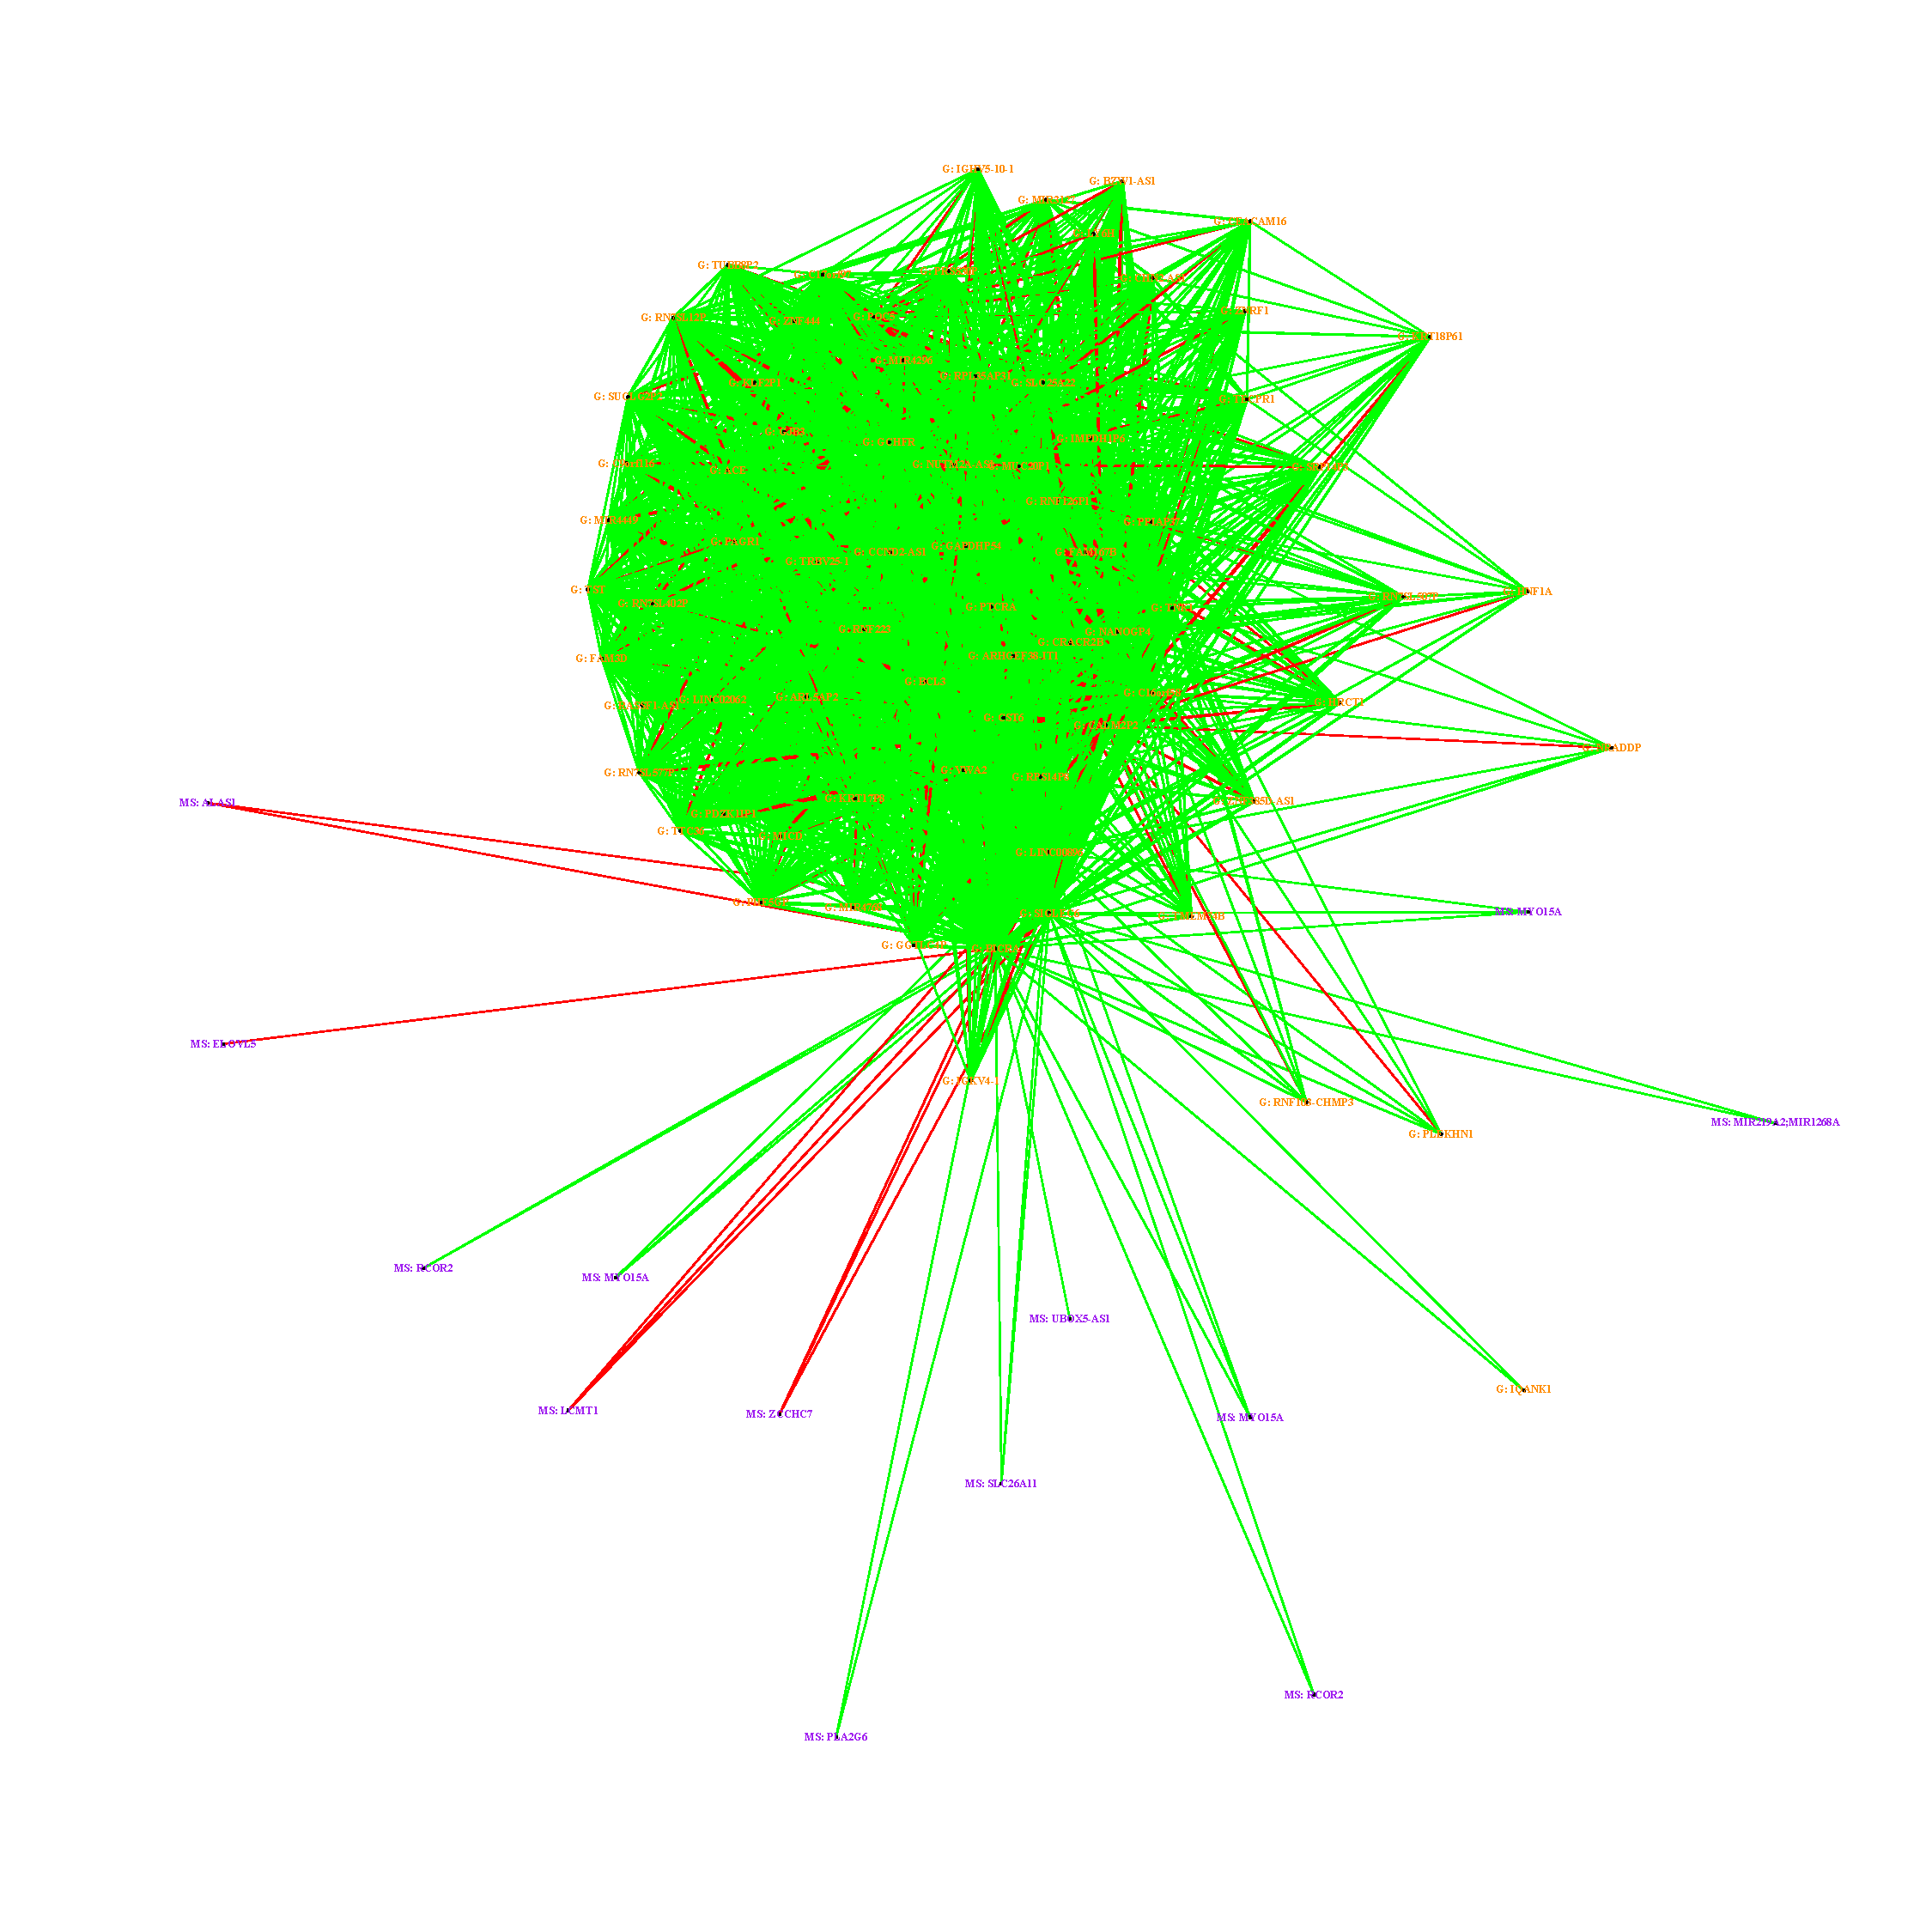
\includegraphics[width=0.7\linewidth]{images/DRDCNet1} \end{center}

\end{frame}

\begin{frame}{SmCCNet identifies key DLBCL genes from literature}
\protect\hypertarget{smccnet-identifies-key-dlbcl-genes-from-literature}{}

{[}INSERT EXAMPLES OF GENES{]}

\begin{longtable}[]{@{}llll@{}}
\toprule
Gene & Function & OMIM & Citation\tabularnewline
\midrule
\endhead
CREBBP & transcription factor & 600140 &
\href{https://www.nature.com/articles/nature09730}{Pasqualucci et al.
(2011)}\tabularnewline
TNK1 & tyrosine kinase & 608076 &
\href{https://www.ncbi.nlm.nih.gov/pmc/articles/PMC2917161/}{May et al.
(2010)}\tabularnewline
BCL3 & NF-\(\kappa\)B inhibitor & 109560 &
\href{https://pubmed.ncbi.nlm.nih.gov/21752100/}{Ibrahim et al.
(2011)}\tabularnewline
ZCCHC7 & TRAMP component & NA &
\href{https://pubmed.ncbi.nlm.nih.gov/30348671/}{Chong et al.
(2018)}\tabularnewline
\bottomrule
\end{longtable}

\end{frame}

\begin{frame}{Conclusions}
\protect\hypertarget{conclusions}{}

{[}INSERT CONCLUSIONS HERE{]}

\end{frame}

\end{document}
